\documentclass[a4paper]{article}

\usepackage[english]{babel}
\usepackage[utf8]{inputenc}
\usepackage{amsmath}
\usepackage{graphicx}
\usepackage[colorinlistoftodos]{todonotes}
\usepackage{hyperref}
\usepackage{subcaption}
\hypersetup{
    colorlinks=true,
    linkcolor=black,
    filecolor=black,      
    urlcolor=blue,
    citecolor=black,
}
\usepackage[labelfont=bf]{caption}
\usepackage[maxbibnames=99,minbibnames=99,sorting=none]{biblatex}
\usepackage{csquotes}
\addbibresource{sample.bib}
\usepackage{sidecap}


\title{\vspace{-2cm}PixelBrush: Art Generation from text with GANs}

\author{Shani Ben Baruch, 
\and Omer Cohen}
\date{}

\begin{document}
\maketitle

\begin{abstract}
Generative adversarial networks (GANs) have been shown to be very effective in generating photo-realistic images. Recent works also allow people to create images from a textual description. In this work, we propose a tool called PixelBrush that generates an artistic image using a given description. The input to our tool is a short text like “a brown horse is standing on the grass”. And the output is a matching image. We based our work on Jaile's project \cite{Zhi2017PixelBrush}. Our entire code is made publicly available at \url{https://github.com/shanibenb/PIxelBrush}.
\end{abstract}


\section{Introduction}
Human excel in tasks the require to create artworks from a giving description. However, for computer algorithms this skill is still limited.

Jaile \cite{Zhi2017PixelBrush}, whom we based our work on, suggested a way of doing that task. He created a tool called PixelBrush. This tool generates an artistic painting from a given description. Jaile uses tensorflow implementation but did not publish his code. We decided to follow Jaile's work, and to create a PyTorch implementation.

There are a couple of challenges around this problem. First, the images that has been used in Jaile's work, have no textual descriptions. He added descriptions using Neuraltalk2 \cite{karpathy2015deep}, and then he manually reviewed them. But obviously, that would not match to our generated descriptions. Second, since there is no code reference for this work, we could not examine for ourselves whether Jaile's results correspond to the results presented in the article.

Some of our results are presented in Figure \ref{fig:gen_images}.


\begin{figure}[!h]
  \begin{minipage}[ht]{0.5\textwidth}\ContinuedFloat
    \caption*{a horse is standing on the grass} \label{fig:horse}
  \end{minipage}\hfill
  \begin{minipage}[ht]{0.5\textwidth}
    \begin{subfigure}[b]{0.2\textwidth}
        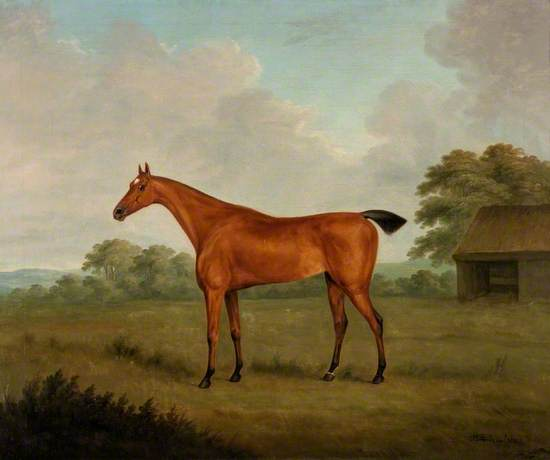
\includegraphics[width=1.22cm, height=1.22cm]{horse_1.jpg}
    \end{subfigure}
    \begin{subfigure}[b]{0.2\textwidth}
        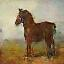
\includegraphics[width=\textwidth]{horse_2.jpg}
    \end{subfigure}
    \begin{subfigure}[b]{0.2\textwidth}
        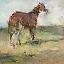
\includegraphics[width=\textwidth]{horse_3.jpg}
    \end{subfigure}
    \begin{subfigure}[b]{0.2\textwidth}
        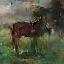
\includegraphics[width=\textwidth]{horse_4.jpg}
    \end{subfigure}
  \end{minipage}
\end{figure}
\vspace*{-7mm}
\begin{figure}[!h]
  \begin{minipage}[ht]{0.5\textwidth}\ContinuedFloat
    \caption*{a man is riding a horse on a dirt field} \label{fig:manhorse}
  \end{minipage}\hfill
  \begin{minipage}[ht]{0.5\textwidth}
    \begin{subfigure}[b]{0.2\textwidth}
        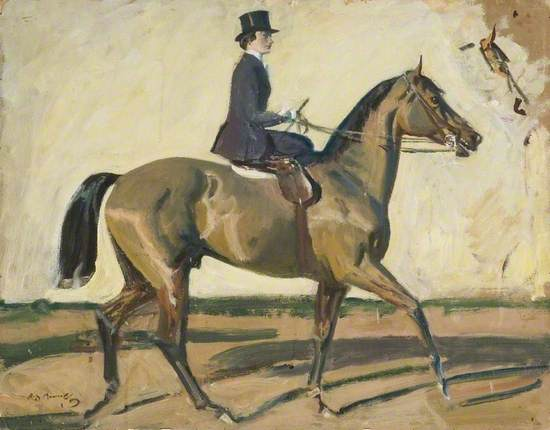
\includegraphics[width=1.22cm, height=1.22cm]{man_1.jpg}
    \end{subfigure}
    \begin{subfigure}[b]{0.2\textwidth}
        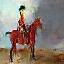
\includegraphics[width=\textwidth]{man_2.jpg}
    \end{subfigure}
    \begin{subfigure}[b]{0.2\textwidth}
        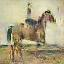
\includegraphics[width=\textwidth]{man_3.jpg}
    \end{subfigure}
    \begin{subfigure}[b]{0.2\textwidth}
        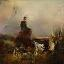
\includegraphics[width=\textwidth]{man_4.jpg}
    \end{subfigure}
  \end{minipage}
\end{figure}
\vspace*{-7mm}
\begin{figure}[!h]
  \begin{minipage}[ht]{0.5\textwidth}\ContinuedFloat
    \caption*{a cow is standing in the field} \label{fig:cow}
  \end{minipage}\hfill
  \begin{minipage}[ht]{0.5\textwidth}
    \begin{subfigure}[b]{0.2\textwidth}
        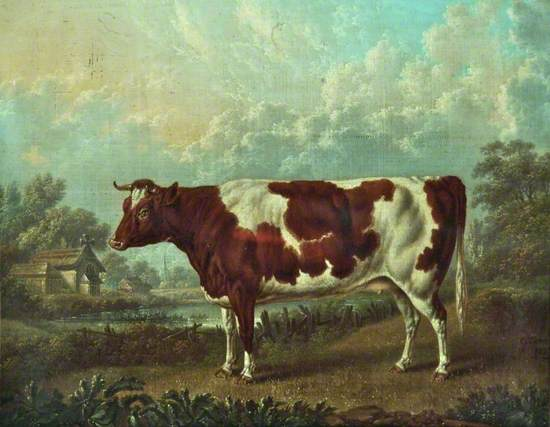
\includegraphics[width=1.22cm, height=1.22cm]{cow_1.jpg}
    \end{subfigure}
    \begin{subfigure}[b]{0.2\textwidth}
        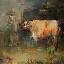
\includegraphics[width=\textwidth]{cow_2.jpg}
    \end{subfigure}
    \begin{subfigure}[b]{0.2\textwidth}
        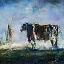
\includegraphics[width=\textwidth]{cow_3.jpg}
    \end{subfigure}
    \begin{subfigure}[b]{0.2\textwidth}
        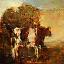
\includegraphics[width=\textwidth]{cow_4.jpg}
    \end{subfigure}
  \end{minipage}
\end{figure}
\vspace*{-5mm}
\begin{figure}[!h]\ContinuedFloat
    \centering
    \caption{Images generated using textual description. First column represent the real images, and the other columns are the generated images.}
    \label{fig:gen_images}
\end{figure}


\section{Related Work} \label{Related_Work}
In the past few years, there were many works which try to generate images using convolutional neural network (CNN) architecture. 

Gatys et al. \cite{gatys2016image} proposed a neural style transfer where new images are been synthesized using a content image and style image. However, this method requires an image as an input. 

Goodfellow et al. \cite{goodfellow2014generative} proposed a methods to generate images given a noise vector. The network proposed contain a generator G and a discriminator D that are been trained together. G synthesizes samples from a target distribution, while D needs to distinguishes between samples generated by G and a training set from the target distribution. The goal of G is to create samples that are classified by D as real samples. 
Radford et al. \cite{radford2015unsupervised} created a successful architecture, based on Goodfellow's work, called deep convolutional generative adversarial network (DCGAN).
Mirza \& Osindero \cite{mirza2014conditional} introduced a new method called conditional generative adversarial network (cGAN) to generate samples from a specific class.

Reed et al. \cite{reed2016generative} were able to generate images based on textual description. They also created a new kind of discriminator called matching-aware discriminator (GAN-CLS), which learn to evaluate whether samples from the generator meet the conditional constraint. They introduced three kind of losses: one, that computes a real image with matching text; second, that computes a synthetic image with arbitrary text; and third, that computes a real image with mismatching text (which the discriminator must learn to score as fake).

Another set of works that generate images from textual description proposed by Zhang et al. \cite{zhang2017stackgan,zhang2017stackgan++}. They were able to generate 256x256 high resolution images.

In our work we aim to generate art images from textual description. This idea is based on Jiale's idea \cite{Zhi2017PixelBrush}. Jaile used Reed et al. \cite{reed2016generative} basic model and change the architecture. Jaile used tensorflow for his work, and did not publish his implementation.

\section{Background}
\subsection{Generative Adversarial Networks}
Generative adversarial networks (GANs) have dramatically expanded the dimension of deep learning research since they were first introduced by Ian Goodfellow et al. \cite{goodfellow2014generative}.

The GAN model consists of two main components: a generator network \(G\) which produces samples \(G(z)\) from the input of random noise \(z\) from distribution \(p_z\), and a discriminator network \(D\) which determines whether a given sample is real from the true data distribution \(p_{data}\) or is artificially created. Both networks are trained simultaneously, and try to optimize the following objective function,
\begin{equation}
    \min_{G}\max_{D}{V(D,G)} = E_{x \sim p_{\mathrm{data}}} [\log{D(x)}] + E_{z \sim p_z} [\log(1-D(G(z)))]
\end{equation}

Conditional GAN \cite{mirza2014conditional} is an extension of GAN where both the generator and the discriminator receive additional information \(c\), yielding \(G(z,c)\) and \(D(z,c)\). This additional information allows the generator to generate images conditioned on that information.

\subsection{Skip-thoughts Text Embedding}
In order to use textual description in our network, we need to convert the description into a vector representation. We use a pre-trained skip-thoughts model proposed by Kiros et al. \cite{kiros2015skip}. This model was trained on the bookCorpus dataset \cite{zhu2015aligning}. 

The skip-thoughts architecture contains one encoder and two decoders. Given a sentence tuple \((s_{i-1},s_i,s_{i+1})\), 
the model takes an input \(s_i\) and tries to predict the previous sentence \(s_{i-1}\) and the following sentence \(s_{i+1}\). 

The are two separate models of the encoder. The first is uni-skip model, which refers to unidirectional encoder with 2400 dimensions. The second is bi-skip model, which refers to a bidirectional model with forward and backward encoders of 1200 dimensions each, the outputs are then concatenated to form a 2400 dimensional vector. There is a third model, combine-skip, which is a concatenation of the uni-skip model and the bi-skip model, resulting a 4800 dimensional vector. In our work we use the combine-skip model.

\section{Dataset}
\subsection{Oxford Painting Dataset}
We use Oxford paintings dataset \cite{Crowley14,Crowley14a} which contains 8629 images in 10 categories: airplane, bird, boat, chair, cow, table, dog, horse, sheep and train. The dataset is split into train, validation and test sets. Because we followed Jaile's work, we merged the different datasets (train, validation and test) and picked around 3200 images from only 4 categories - cow, dog, horse and sheep. 85\% of the merged dataset has been used for training, and the other 15\% for testing. Some
sample paintings are shown in Figure \ref{fig:oxford}.

\begin{figure}[ht]
    \centering
    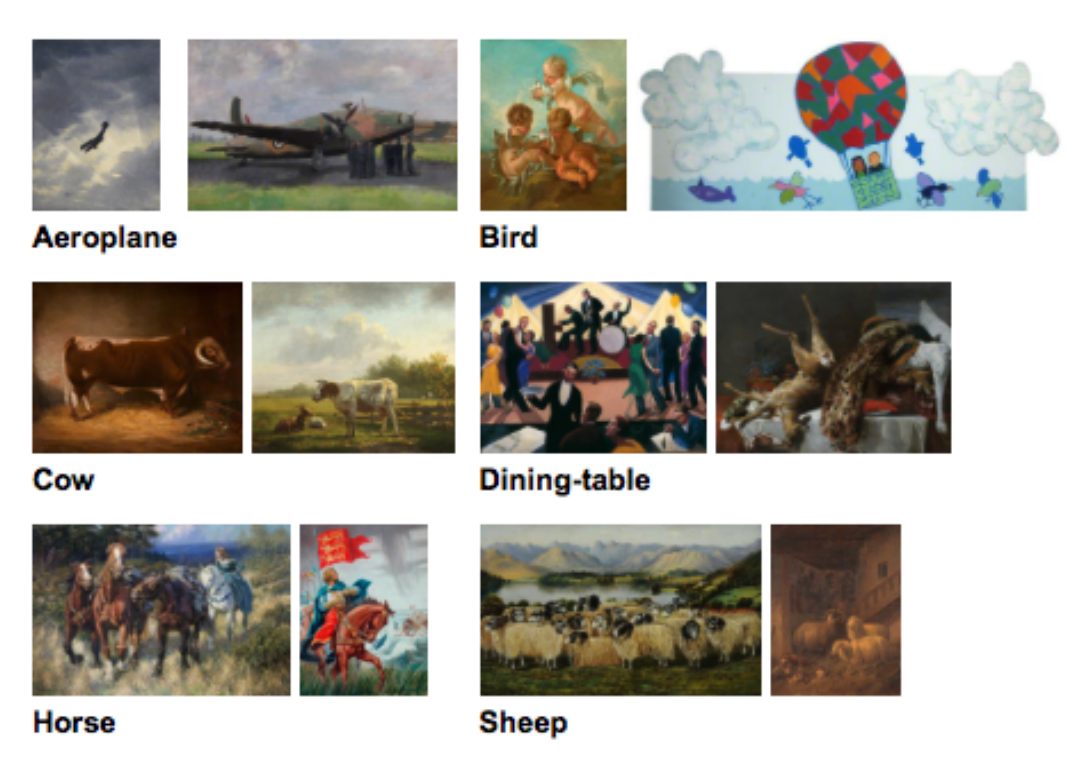
\includegraphics[width=0.9\textwidth]{oxford.png}
    \caption{Sample images from Oxford Paintings dataset}
    \label{fig:oxford}
\end{figure}

\subsection{Adding Descriptions}
This dataset only contains images with titles and categories. However, this is not enough to generate artwork, and we also need textual description for each image.
As proposed by Jaile we used a two-step solution to create those descriptions. First, we generate descriptions using Neuraltalk2 \footnote{https://github.com/raoyongming/neuraltalk2.pytorch}, a pre-trained network (trained on MSCOCO dataset), proposed by Karpathy et al. \cite{karpathy2015deep}. Second, we manually reviewed all the generated descriptions and fixed the defects.

\section{Methods}
\subsection{Network Architecture}
As discussed before, we followed the architecture proposed by Jaile \cite{Zhi2017PixelBrush}, who drew it from Reed et al. \cite{reed2016generative}. We used a PyTorch implementation of Reed's article as our baseline \footnote{https://github.com/aelnouby/Text-to-Image-Synthesis}. The architecture is presented in Figure \ref{fig:Network}.

First, we create text embedding from a given description, using skip-thoughts model. Second, we concatenate that embedding with random noise vector \(z\). And third, we train a generative adversarial network. The generator aims to create images conditioned on text description. The discriminator aims to determine whether the input images are real or fake based or their descriptions (see GAN-CLS in section \ref{Related_Work} for more details).

 \begin{figure}[ht]
    \centering
    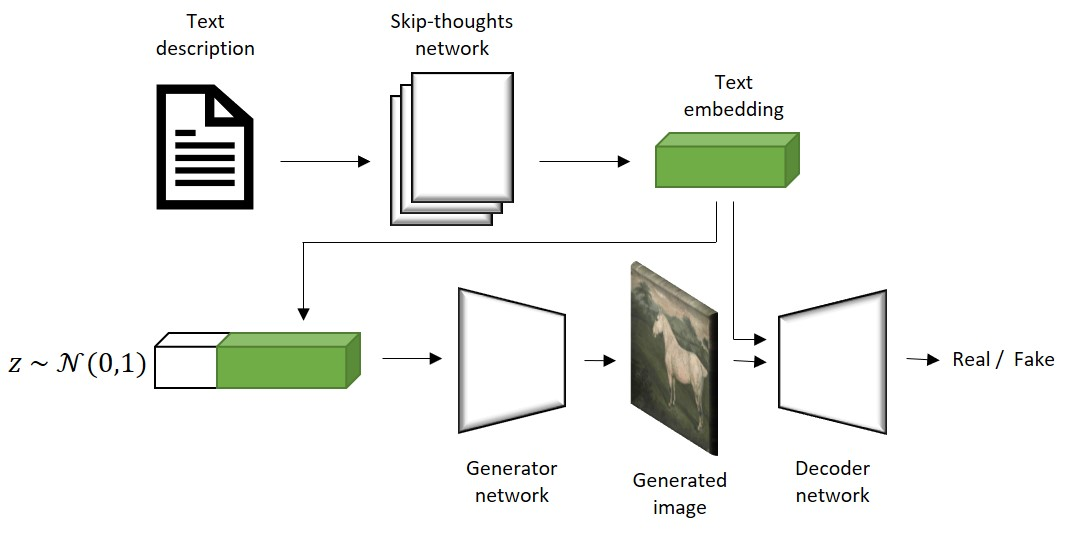
\includegraphics[width=\textwidth]{network.jpg}
    \caption{Overview of the network architecture}
    \label{fig:Network}
\end{figure}

\subsection{Generator architecture}\label{generator}
\begin{table}[!ht]
    \centering
    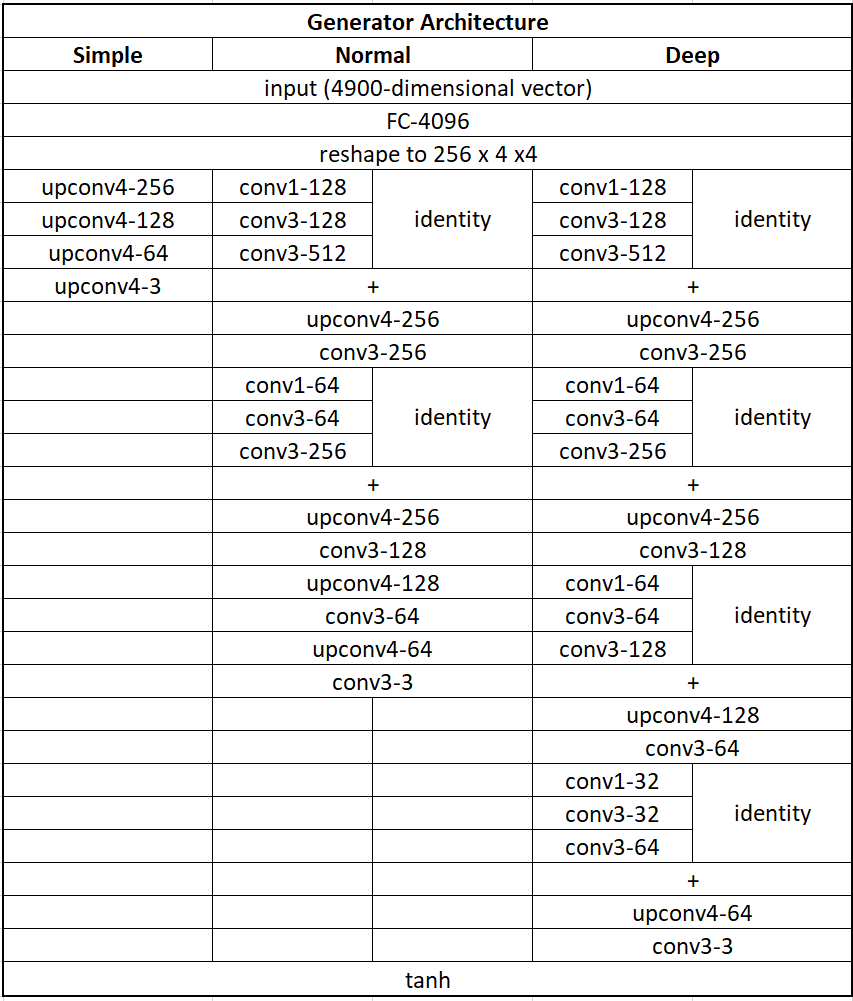
\includegraphics[trim={0.03cm 0.01cm 0.01cm 0.03cm},clip,width=\textwidth]{generator.jpg}
    \caption{Generator network architectures (simple, normal and deep). The (up)conv layers denote as $"(up)conv\langle filter size \rangle - \langle number of channels\rangle"$}
    \label{tab:generator}
\end{table}
There are 3 different kinds of generators we built: simple, normal and deep (see Table \ref{tab:generator} for more details). The input for each generator is a concatenation of a random noise vector with 100 dimensions and a text embedding with 4800 dimensions. The output is an image of size 3x64x64.

We use transpose convolution with stride 2 for up-sampling, and convolutional layers with stride 1. Each layer, except the last layer, follow by batch normalization and ReLU activation. The method for creating the normal and deep networks is similar to ResNet \cite{he2016deep}, which allows us to create deeper networks.


\subsection{Discriminator architecture}
The discriminator is built from convolutional layers follow by batch normalization and leakyReLU activation. The last convolutional layer is only follow by a sigmoid layer. The input is a 3x64x64 image and a text embedding vector, and the output is a score that indicated whether the image is real or fake (see Figure \ref{fig:Disc}).

 \begin{figure}[ht]
    \centering
    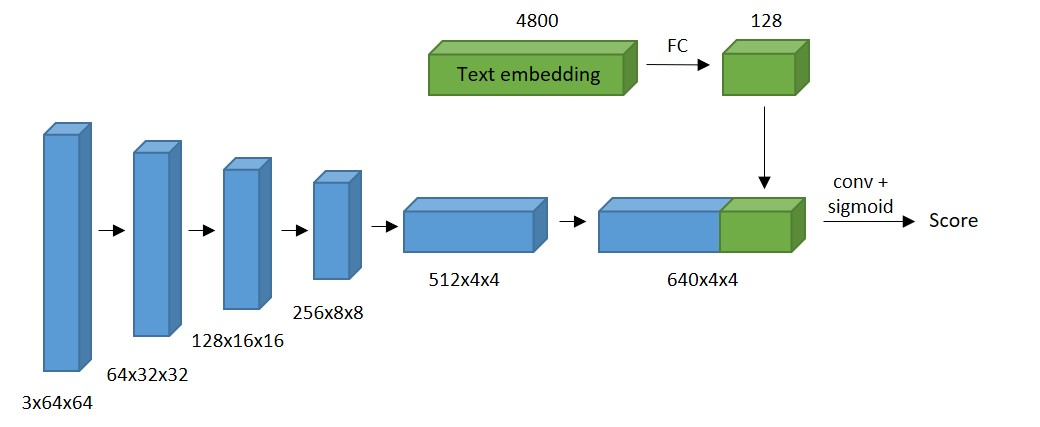
\includegraphics[width=\textwidth]{disc.jpg}
    \caption{Overview of discriminator architecture}
    \label{fig:Disc}
\end{figure}


\section{Experiments}
\subsection{Evaluation metrics}
It is difficult to evaluate performance on GAN models. For this project we follow Jaile suggestion and choose inception score (IS) \cite{salimans2016improved},
\begin{equation}
    I = \exp({E_x D_{KL} (p(y|x)||p(y)))}, 
\end{equation}
where $x$ denote the generated image, and $y$ is the label predicted by the IS. The intuition behind this metric  is that good models should generate diverse but meaningful images. Therefore, the KL divergence between the marginal distribution $p(y)$ and the conditional distribution $p(y|x)$ should be large.

\subsection{Comparison between different generators}
To understand how the depth affects the generated images, we trained our network with three different architectures: ”simple”, ”normal” and ”deep” as denoted in \ref{generator}.

From Table \ref{tab:generator} we can see that the inception score is roughly increases with the number of training iterations. In addition, inception score increases when the generator's architecture goes deeper. This results match Jaile's results in his paper.


\subsection{Comparison against baseline}
We tested our work against a GAN model that does not use textual descriptions. We follow the network of DCGAN \cite{radford2015unsupervised}, and compared it to our "simple" generator architecture. Results after 250 epochs are presented in Table \ref{tab:inception_DCGAN} and in Figure \ref{fig:DCGAN}.

We can see that like Jaile's results, the "simple" architecture created better images than DCGAN architecture. This reflects both in the inception score and in the visibility of the images themselves. These results support the intuition that using the help of the descriptions, conditional GAN generate objects that look more real. However, DCGAN does not use descriptions so everything is more likely to be mixed together.


\begin{figure}[ht]
    \centering
    \begin{subfigure}[b]{0.45\textwidth}
        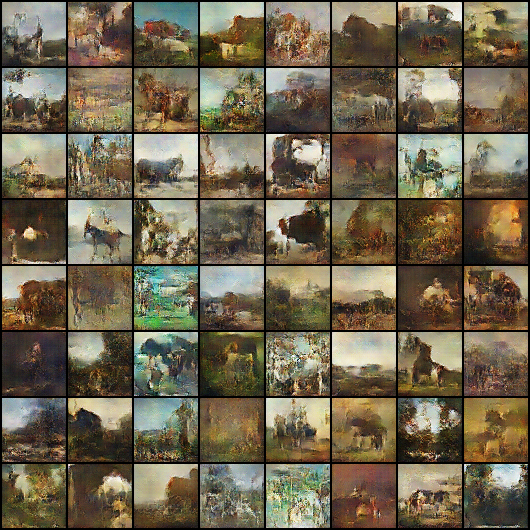
\includegraphics[width=\textwidth]{vanillaGAN.jpg}
    \end{subfigure}
    \hspace{0.5cm}
    \begin{subfigure}[b]{0.45\textwidth}
        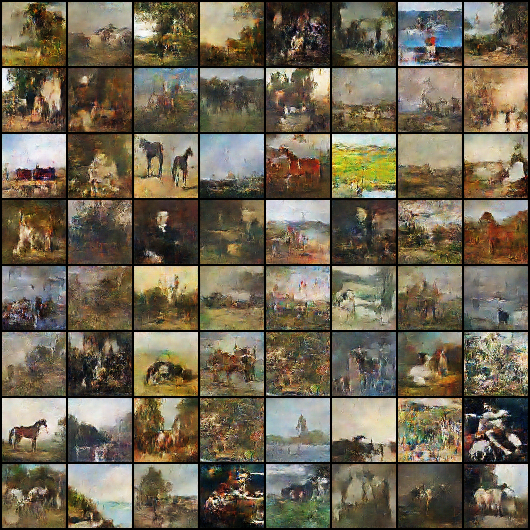
\includegraphics[width=\textwidth]{simpleGAN.jpg}
    \end{subfigure}
    \caption{Comparison between DCGAN and "simple" architecture. images generated after 250 epochs. Left: images generated using DCGAN. Right: images generated using our "simple" architecture.}\label{fig:DCGAN}
\end{figure}

\begin{table}[!ht]
    \centering
    \begin{tabular}{c|c}
        method & inception score\\
        \hline
        DCGAN & $1.84 \pm  0.25$ \\
        Simple generator & $2.87 \pm 0.10$
    \end{tabular}
    \caption{Inception score for DCGAN and "simple" architecture after 250 epochs. Higher inception score means better image quality.}
    \label{tab:inception_DCGAN}
\end{table}

\begin{table}[!ht]
    \centering
    \begin{tabular}{c|c|c|c}
        epochs & simple & normal & deep\\
        \hline
        20 & $1.55 \pm  0.05$ & $\boldsymbol{2.02 \pm  0.11}$ & $1.96 \pm  0.13$ \\
        40 & $1.87 \pm 0.10$ & $1.96 \pm 0.15$ & $\boldsymbol{2.09 \pm 0.12}$ \\
        60 & $1.88 \pm 0.14$ & $2.08 \pm 0.19$ & $\boldsymbol{2.29 \pm 0.19}$ \\
        80 & $1.93 \pm 0.12$ & $2.20 \pm 0.13$ & $\boldsymbol{2.24 \pm 0.13}$ \\
        100 & $2.07 \pm 0.10$ & $1.97 \pm 0.10$ & $\boldsymbol{2.27 \pm 0.19}$
    \end{tabular}
    \caption{Inception score for 3 kinds of generator networks. Higher inception score means better image quality.}
    \label{tab:inception_generators}
\end{table}

\section{Conclusion}
This work is a PyTorch implementation of a tool called PixelBrush, which invented bu Jaile \cite{Zhi2017PixelBrush}. This tool creates an artistic image using a given textual description. The architecture of this model is based on a conditional GAN. We showed that by adding a description as a condition, we can get more recognizable images. We also showed that better quality images can be created by adding more layers to the generator.

\section{Future Work}
Our image resolution in currently limited to 64x64. It would be interesting to use StackGAN or StackGAN++ by Zhang et al. \cite{zhang2017stackgan,zhang2017stackgan++}, and try to increase the resolution to 256x256. It would be also interesting to add more descriptions to the images using different methods, like the one created by Vinyals et al. \cite{vinyals2017show}.

\printbibliography
\end{document}
